Les quaternions unitaires représentent l'\emph{espace mathématique} des rotations en trois dimensions de façon relativement simple. On peut comprendre la correspondance entre les rotations et les quaternions en commençant d'abord par se faire une idée intuitive de l'espace des rotations lui-même.
Deux rotations d'angles différents et d'axes différents dans l'espace des rotations. La norme du vecteur est liée à l'amplitude de la rotation.

Chaque rotation en trois dimensions consiste à tourner d'un certain angle autour d'un certain axe. Quand l'angle est nul, l'axe n'a pas d'importance, de telle façon qu'une rotation de zéro degré est un simple point dans l'espace des rotations (c'est la rotation identité). Pour un angle petit mais non nul, l'ensemble des rotations possibles est une petite sphère entourant la rotation identité, où chaque point de la sphère représente un axe pointant dans une direction particulière (comparez avec la sphère céleste). Des rotations d'angles de plus en plus grands s'éloignent progressivement de la rotation identité, et nous pouvons nous les représenter comme des sphères concentriques de rayons croissants. Par conséquent, au voisinage de la rotation identité, l'espace abstrait des rotations ressemble à l'espace ordinaire en trois dimensions (qui peut également être vu comme un point central entouré de sphères de différents rayons. La ressemblance s'arrête là : lorsque l'angle de rotation dépasse \ang{180}, les rotations suivant les différents axes cessent de diverger et commencent à nouveau à se ressembler, pour finir par devenir identiques (et égales à la rotation identité) lorsque l'angle atteint \ang{360}.

\begin{figure}[ht]
	\centering
	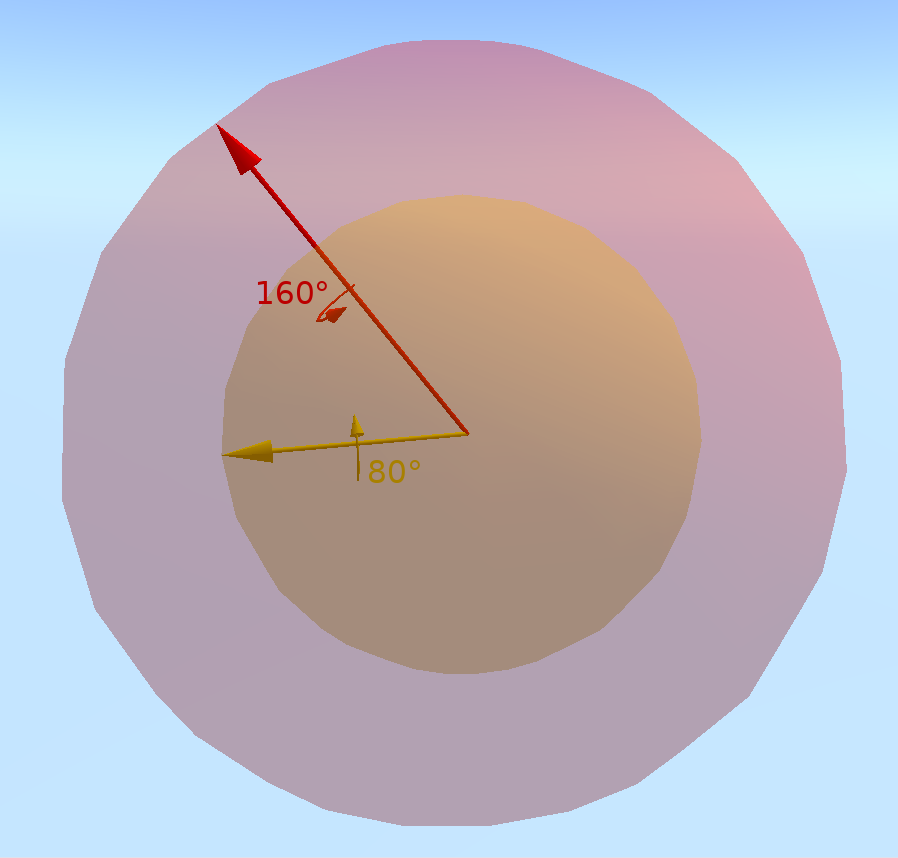
\includegraphics[width=5cm]{ressources/espace_rotations}\hfill
	\caption{Deux rotations d'angles différents et d'axes différents dans l'espace des rotations. La norme du vecteur est liée à l'amplitude de la rotation.}
	\label{espace_rotations}
\end{figure}

L'hypersphère des rotations pour les rotations d'axes horizontaux (axes compris dans le plan xy).
On constate un phénomène analogue à la surface d'une sphère. Si nous nous plaçons au pôle Nord et traçons à partir de là des lignes droites (en fait, des méridiens) dans plusieurs directions, elles divergeront puis convergeront à nouveau au pôle Sud. Des cercles concentriques de rayon croissant dessinés autour du pôle Nord (des parallèles) finiront par s'effondrer en un point au pôle Sud une fois que l'on a parcouru la distance entre les pôles. On peut assimiler les différentes directions à partir du pôle (c'est-à-dire les différents méridiens) aux différents axes de rotations et les différentes distances au pôle Nord aux différents angles : on a ainsi une analogie de l'espace des rotations. Mais la surface de la sphère est en deux dimensions alors que les \emph{axes} de rotation utilisent déjà trois dimensions. L'espace des rotations est donc modélisé par une sphère de dimension 3 dans un espace à 4 dimensions (une hypersphère). Nous pouvons penser à la sphère ordinaire comme à une section de l'hypersphère, de la même façon qu'un cercle est une section de sphère. On peut prendre la section pour représenter, par exemple, uniquement les rotations d'axes dans le plan $xy$ (voir illustration ci-contre). On remarque que l'angle de la rotation est deux fois la différence de latitude avec le pôle Nord : en effet, les points de l'équateur représentent des rotations de \ang{180}, pas de \ang{90}, et le pôle Sud représente la rotation identité de \ang{360}, et pas le demi-tour de \ang{180}.

Le pôle Nord et le pôle Sud représentent la même rotation, et en fait cela s'applique à n'importe quelle paire de points aux antipodes l'un de l'autre : si un point correspond à une rotation d'angle $\alpha$ autour de l'axe dirigé par le vecteur $\vv{v}$, l'autre point correspond à une rotation d'angle $\text{\ang{360}} - \alpha$ autour de l'axe dirigé par le vecteur $\vv{v}$. En fait, l'espace des rotations n'est pas l'hypersphère elle-même, mais l'hypersphère où l'on identifie les points aux antipodes l'un de l'autre. Mais dans un but de simplification, nous pouvons penser aux rotations comme à des points de la sphère en dimension 4, même si la moitié de ces points est redondante (revêtement double).

\begin{figure}[ht]
	\centering
	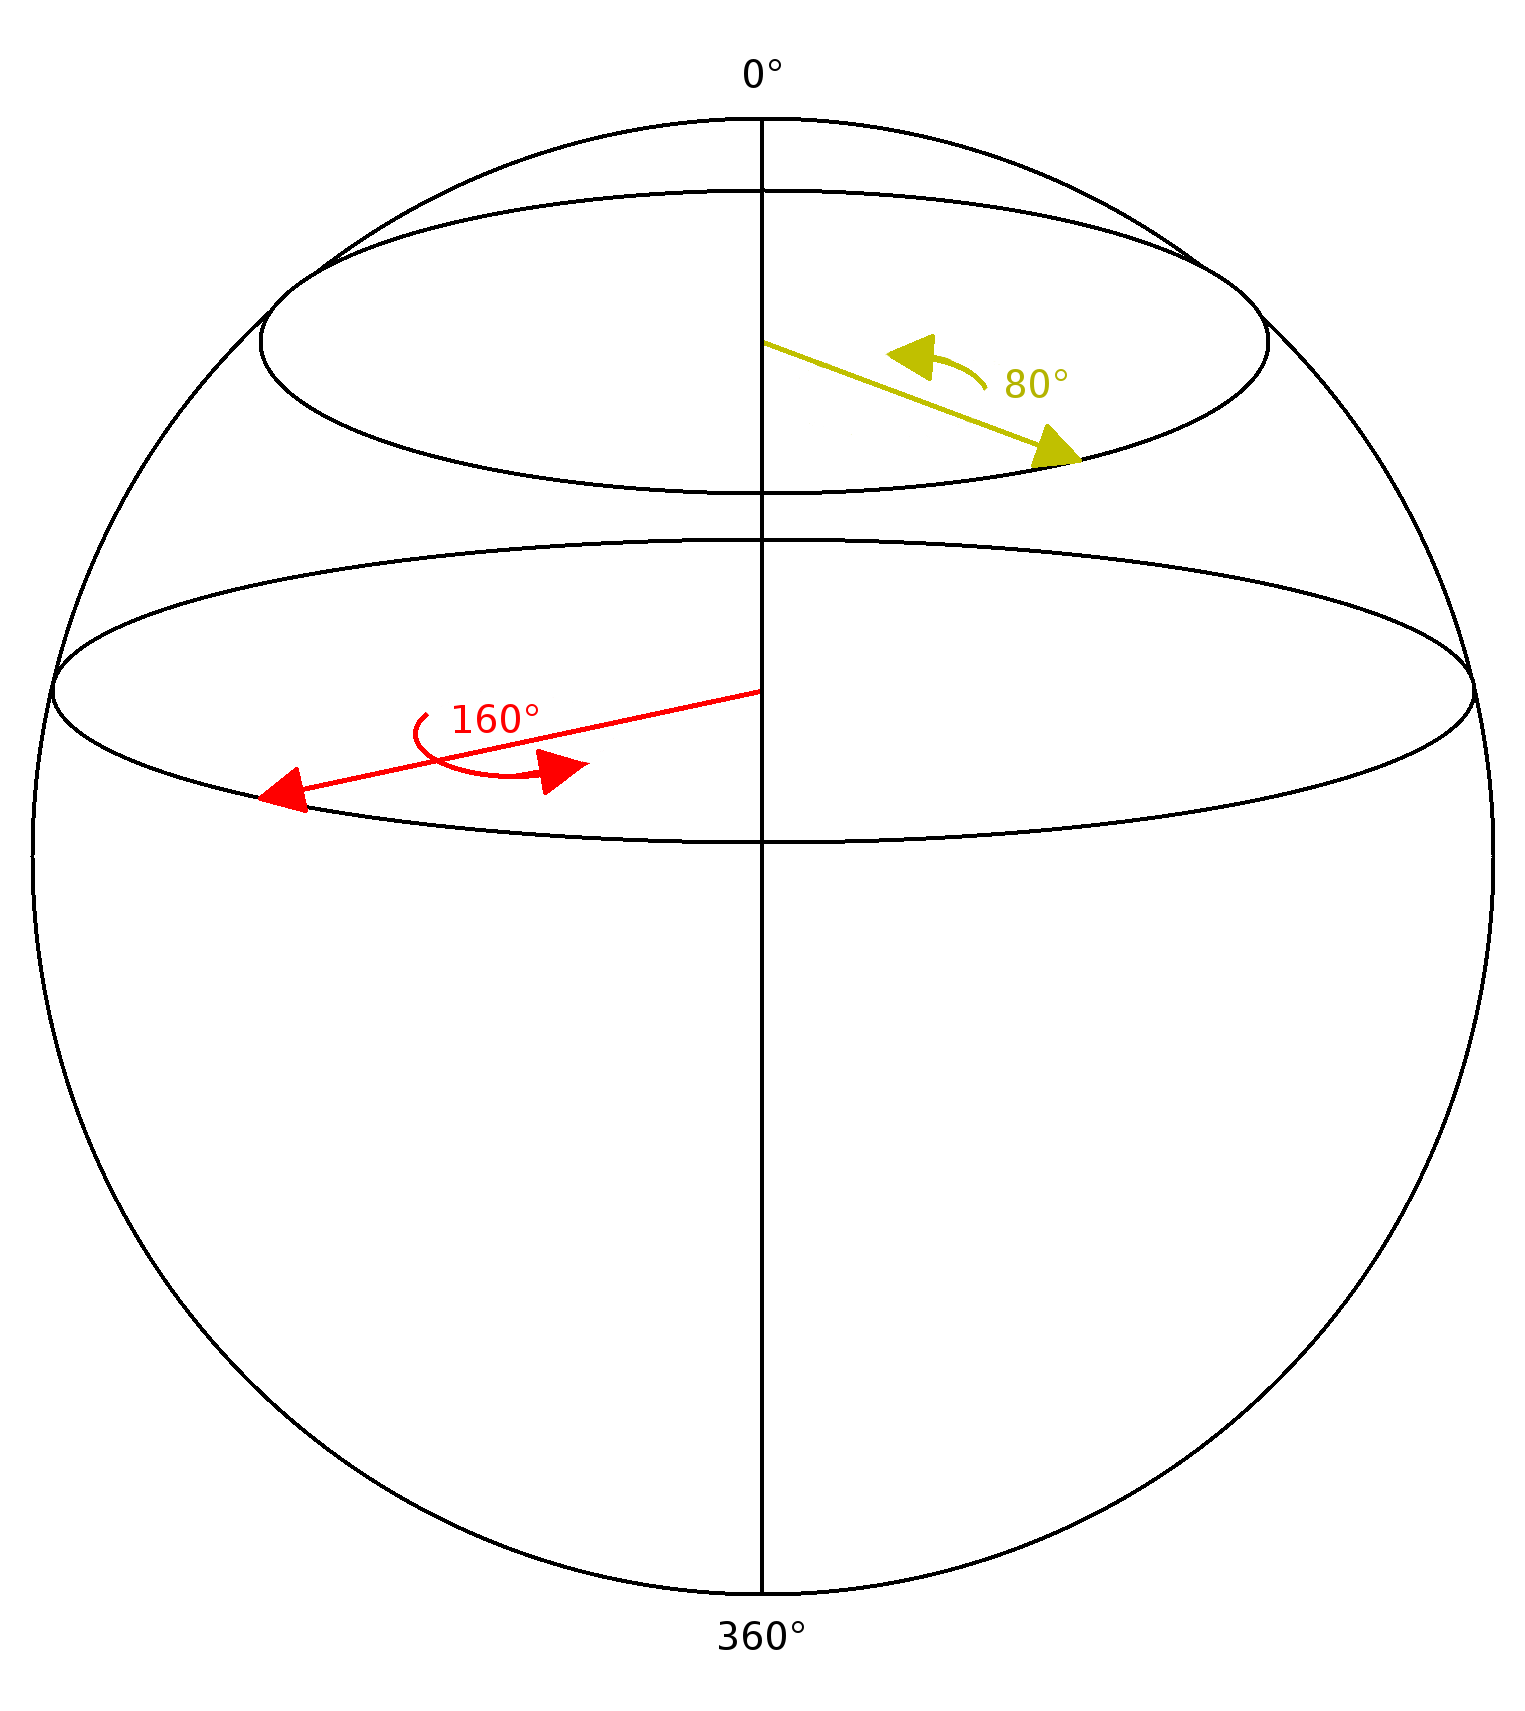
\includegraphics[width=5cm,height=4cm]{ressources/hypersphere_rotations}\hfill
	\caption{L'hypersphère des rotations pour les rotations d'axes horizontaux (axes compris dans le plan $xy$).}
	\label{hypersphere_rotations}
\end{figure}